\section{Ownership Assignment}
\label{section:ownership}


We formulate the last-mile search problem in terms of \textit{locations}, which are searchable entities that 'own' or contain any number of \textit{objects}. Motivated by the way humans tend to recall memories of locations....................add some details for context?..........................., we designed \emph{GESTALT} to enable users to search for locations using their objects (and optionally their spatial relationships) as the search conditions (i.e. a location that contains <object1, object2, etc.>, or a location that contains <object1 Northeast of object2>). To enable these types of queries, \emph{GESTALT} must associate objects with their parent locations.
We call this problem \textit{Object Ownership Assignment}, and define it as follows:

...........definition latex formatting.................... Given a collection of locations and objects within a region, \emph{Ownership Assignment} seeks to correctly assign each object to its 'parent' location. This amounts to a clustering problem where points (objects) are assigned to centroids (locations) that are known apriori. The objects are not uniformly distributed across locations, and some locations may not have tagged objects associated with them. 


In the absence of reliable crowd-sourced data linking objects to their parent locations, the ownership assignment problem necessitates an unsupervised solution to scale to any nontrivial number of locations and objects. Further, the human eye does not see the world in regular grid lines such as on a map, and so the ownership assignment process is naturally inexact, and objects are 'shared' between locations where appropriate. For example, a winery may have a shed out back that is visible both from that winery, and from a neighboring one. In this case, the object can be useful when searching for either location. We address this aspect of the problem with fuzzy assignment (subsection \ref{subsection:fuzzy_asn}).


\subsection{Datasets and Metrics}

We perform the Ownership Assignment task on two datasets: the hand-labeled Swan Valley Wineries dataset alone and a \textit{Combined} dataset that includes all of the object and location tags from the Swan Valley Wineries dataset in addition to the noisy object tags from the Flickr dataset and the crowd-sourced object tags from the OSM dataset.
Since we have ground truth labels for the winery locations and their objects in the Swan Valley dataset, we report both precision and recall on this dataset.
The Combined dataset presents a more realistic and challenging scenario for Ownership Assignment than the Swan Valley Wineries dataset alone, given its larger set of locations and very large set of object tags to assign to those locations. However, since the Combined dataset includes noisy tags for which we have no ground truth labels, we do not report precision on the Combined dataset. Instead, we measure only the recall on the same set of Winery locations and their known objects that were hand-labeled as part of the Swan Valley dataset. The Combined dataset tests how well the recall performance of our Ownership Assignment method holds up to additional noise and more densely packed objects and locations.

The Swan Valley Wineries dataset consists of 31 wineries retrieved from OSM and ................\~150 objects hand-labeled across 6 of those 31 locations with ground-truth labels. Table \ref{table:clustering} contains the recall (and precision, where applicable) on those locations and objects.


\subsection{Method- Object Ownership Assignment}
ALGORITHM ObjectOwnershipAssignment
1. Use DBSCAN to group objects into clusters, or assign them to the null cluster
2. For objects that did cluster (i.e. objects not assigned to the null cluster):
    3. Calculate the centroids of the clusters
    4. Calculate the confidence scores for each object's assignment to the cluster as 1 - normalized distance from object to centroid of its cluster
5. Set confidence score to 0.5 for objects assigned to the null cluster 
6. Map the centroids to the nearest location


After clustering the objects, we determine the centroids of the relevant object clusters, calculate the confidence scores in the object-cluster assignments, and then map the cluster centroids to their nearest known location tags. 
When calculating the confidence scores, we normalize the object-centroid distances (omitting objects in the null cluster, which has no meaningful centroid and would skew the normalization). 
This confidence score (between 0 and 1) measures how far a given object is from it's cluster's centroid, assigning higher scores to objects near the centroid and lower ones to objects far from the centroid. 
We take this approach rather than using a static threshold parameter (like within x distance) to account for variety in object density of the region under search. 
We adopt the convention of assigning null cluster objects a confidence score of 0.5 since these objects are deemed to be noise and are not relevant or useful in finding locations.

The benefit of using DBSCAN in the Object Ownership Assignment context is that it acts as a noise reducer, filtering out objects which do not belong to any locations (i.e. a mis-tagged singular object with nothing else around it for miles in any direction). 
The downside of using DBSCAN in this context is that it determines the centroids of the object clusters based on the object density, and then we must map those to our known location centroids in a post-processing step. 
Ideally, a better solution would start with the centroids and cluster around them. 
The DVBSCAN algorithm Ram et al. proposed in 2010 presents a promising direction to resolve this problem~\cite{Ram2010}, while retaining the noise reduction effects of traditional DBSCAN. 
We leave a detailed comparison of Object Ownership Assignment techniques as an interesting avenue of future study for the last-mile search problem.
 
%In step 6: Given a KD tree constructed from location point coordinates, a nearest neighbor search on the KD tree yields the location nearest to the centroid and it is assigned ownership of that cluster

\subsection{Method- Fuzzy Object Ownership Assignment} \label{subsection:fuzzy_asn}
..................TODO NSCH:............ Write up ALGO for fuzzy clustering of objects to locations, where objects can be assigned to multiple locations with some probability p.

Of note, because the human eye can see over property boundaries and other invisible lines on maps, we can accept a small margin of error where objects from neighboring locations might be mislabeled. For example, perhaps there is a large red shed at the back of a location's property that is not visible to the main part of the parent location but is clearly visible to the neighboring location.
There will also exist some objects which plausibly could be seen and remembered by patrons of several locations, for example, a lake or a giant statue. 
This multiple-ownership situation is one of the driving requirements for implementing concept mapping to extract additional discriminatory information between locations based on the geospatial layout of objects.


\subsection{Results}
This section discusses the empirical analysis of the clustering methods tested during the implementation of the Ownership Assignment process. 

\begin{table}[h!]
	\begin{center}
		\begin{tabular}{ |c|c|c|c|c|c| } 
			\hline
			Dataset & Total Locs & Total Objs & Method & Precision & Recall \\
			\hline
			\multirow{2}{9em}{Swan Valley Wineries } 
                & 31 & ?? & Exact & $??$ & $??$  \\ 
			& 31 & ?? & Fuzzy & $??$ & $??$  \\ 
			\multirow{2}{9em}{Combined} 
                & ??? & ??? & Exact & - & $??$  \\ 
			& ??? & ??? & Fuzzy & - & $??$  \\ 
			\hline
		\end{tabular}
		\label{table:clustering}
		\caption{............................Combined means hand-labeled Swan Valley Wineries dataset tags and Flickr noisy object-detected tags which we have no ground truth for. We only report recall for the combined dataset since the hand-labeling was not exhaustive, and some results forom the noisy data may be correct but not in the ground truth.}
	\end{center}
\end{table}


\begin{figure*}[ht]
\label{fig:cmeans}        
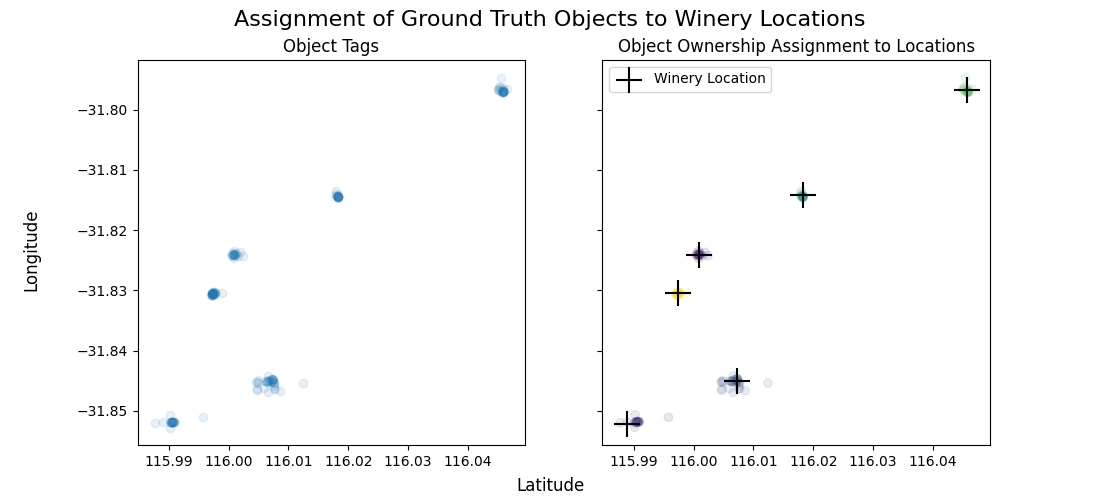
\includegraphics[width=\textwidth]{gestalt_cmeans.png}
\centering
\caption[width=\textwidth]{............}
\end{figure*}


\subsection{Scalability}
The ownership assignment process needs to be unsupervised to enable scaling to millions of object tags. 

- complexity analysis

- present timings/ etc.





%Examining the errors reveals the following insights about each clustering technique. 
%\textbf{When K-Means clusters incorrectly, labels are still correct.} When $K$ exceeds the number of clusters, it fragments the actual clusters. 
%However, in ideal conditions like the Wineries Dataset, where locations are separated, the centroids of these cluster fragments are still closest to the correct location. 
%As a consequence, they are correctly labeled despite being incorrectly clustered. We expect the accuracy will drop when locations are more densely packed. However, when we aim to process all objects and locations in a region concurrently, the number of clusters will likely approach the number of locations, and the issue will be less pronounced. 


%The second, more common (and more challenging approach) formulates an unsupervised learning problem using clustering libraries from \textit{scikit-learn}\footnote{\href{https://pypi.org/project/scikit-learn/}{Scikit-Learn PyPI Repo}}. 

%Ownership assignment is the unsupervised process through which objects are associated with locations. 
%Objects need to be associated with locations in \textit{GESTALT} because for the \textit{concept mapping} process and \textit{search} subsystem to work, they need to know which objects belong to each location.
%For example, assuming two adjacent wineries, a fountain between them would be west of one but east of the other. The mapping will be incorrect unless it is clear which winery it belongs to. 
%Similarly, for search, the underlying idea for \textit{GESTALT} is that people will remember particular objects at locations and use them as clues to find them again. Without an accurate object-to-location assignment, the search functionality will not work. 
 
%The Ownership Assignment process accepts two inputs, a collection of locations with their coordinates and a collection of objects with their coordinates. 
%The process works to assign each object to its parent location. 
%The process ends when objects are mapped to their parent locations. 